\documentclass[a4paper]{article}

\makeatletter
\usepackage{amsfonts}
\usepackage{amsmath}
\usepackage{amssymb}
\usepackage{amsthm}
\usepackage{bm}
\usepackage[english]{babel}
\usepackage{booktabs}
\usepackage[margin = 10pt, font = small, labelfont = bf]{caption}
\usepackage{fancyhdr}
\usepackage{graphicx}
\usepackage{xcolor}
\usepackage{mathtools}
\usepackage{microtype}
\usepackage{multirow}
\usepackage{pdflscape}
\usepackage{pgfplots}
\usepackage{siunitx}
\usepackage{tabularx}
\usepackage{tikz}
\usepackage{sectsty}
\usepackage{derivative}
\usepackage{braket}
\usepackage[colorlinks=true
   ,urlcolor=blue
   ,anchorcolor=blue
   ,citecolor=blue
   ,filecolor=blue
   ,linkcolor=blue
   ,menucolor=blue
   ,linktocpage=true
   ,pdfa=true
]{hyperref}

\pagestyle{fancyplain}
\fancyhead[R]{Oscar Emil Sommer \\
A. Anand}
\fancyfoot{}
\fancyfoot[C]{\thepage}

\renewcommand{\@dotsep}{10000} %No dots in ToC
\allsectionsfont{\bfseries\sffamily} %Sections are bold sans serif



% Theorem-like environments
\theoremstyle{definition}
\newtheorem*{axiom}{Axiom}
\newtheorem*{aprx}{Approximation}
\newtheorem*{claim}{Claim}
\newtheorem{theorem}{Theorem}[section]
\newtheorem{corollary}[theorem]{Corollary}
\newtheorem{definition}{Definition}[section]
\newtheorem{conjecture}{Conjecture}
\newtheorem*{example}{Example}
\newtheorem*{exercise}{Exercise}
\newtheorem*{fact}{Fact}
\newtheorem*{remark}{Remark}
\newtheorem*{method}{Method}
\newtheorem{lemma}[theorem]{Lemma}
\newtheorem{proposition}[theorem]{Proposition}


\newtheorem*{principle}{Principle}
\setcounter{tocdepth}{2}
\makeatother

\author{Oscar Emil Sommer}
\usetikzlibrary{calc}
%Upright symbols
\renewcommand{\i}{\mathrm{i}}
\newcommand{\e}{\mathrm{e}}
\newcommand{\p}{\partial}
%Vector formatting
\renewcommand{\Vec}[2]{\left(\begin{array}{c} {#1} \\ {#2} \end{array}\right)}


%Common sets
\newcommand{\R}{\mathbb{R}}
\newcommand{\Z}{\mathbb{Z}}
\newcommand{\N}{\mathbb{N}}
\newcommand{\Q}{\mathbb{Q}}
\newcommand{\C}{\mathbb{C}}
\newcommand{\M}{\mathcal{M}}

%Common Groups
\newcommand{\SU}{\mathrm{SU}}
\newcommand{\SL}{\mathrm{SL}}
\newcommand{\GL}{\mathrm{GL}}
\newcommand{\Orth}{\mathrm{O}}
\newcommand{\SO}{\mathrm{SO}}
\newcommand{\U}{\mathrm{U}}
\renewcommand{\Im}{\operatorname{Im}}
\renewcommand{\Re}{\operatorname{Re}}


\newcommand{\su}{\mathfrak{su}}
\newcommand{\gl}{\mathfrak{gl}}
\newcommand{\so}{\mathfrak{so}}
%Common stylistic variable

\newcommand{\ep}{\epsilon}
\newcommand{\var}[1]{\delta #1\,}
\newcommand{\dd}[1]{\mathrm{d}#1\,}
\newcommand{\oes}[1]{\textcolor{red}{#1}}
\newcommand{\oesimp}[1]{\textcolor{blue}{#1}}
\newcommand{\vb}{\mathbf}
\newcommand{\ketbra}[2]{\ket{#1}\!\!\bra{#2}}
\newcommand{\Tr}{\operatorname{Tr}}
\newcommand{\up}{\uparrow}
\newcommand{\down}{\downarrow}

\begin{document}
Open quantum dynamics of quantum optical many body systems

\section{Lecture 1}
By Massimo Palma

No microscopic derivation, but more useful persepctive: 
**collision model.**

Model your environment as consisting of several subsystem think of them as
particles.

Your system collides with each of the subsystem of the environment sequentially,
pairwise collisions.


\begin{example}[Micromason]
Cavity inject stream of atom such that only 1 atom is inside at a time. Beam of
atoms acts as environment, and by construction is collision model.
\end{example}
Collision model allow us to follow  both environemnt and system, in contrast to
more standard master equation where you only follow reduced dynamics.

Can follow quantum trajectory :)

Useful: 
 - Want to follow trajectory or environment.



 \subsection{Technical details}
Interaction picture

System density $\rho=r$, 
Environment $\eta=e$.
\begin{center}
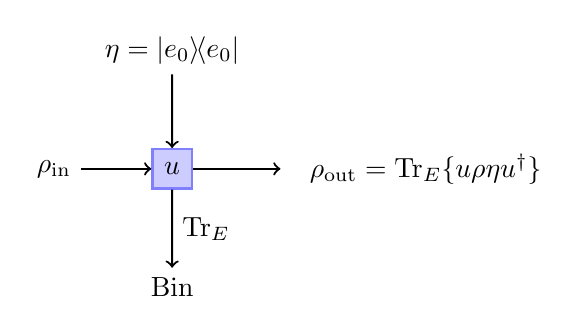
\begin{tikzpicture}[scale=1.5]
    \node[](in){$\rho_\mathrm{in}$};
    \node [rectangle,fill=blue!20,draw=blue!50,thick,minimum height=0.5cm,minimum
        width=0.5cm] (int) at ($(in)+(1,0)$) {$u$};
    \node [](env) at ($(int)+(0,1)$){$\eta=\ketbra{e_0}{e_0}$};
    \node [label=east:{$\rho_\mathrm{out}=\Tr_E\{u\rho\eta u^\dagger\}$}](out) at ($(int)+(1,0)$){};
    \node [](bin) at ($(int)-(0,1)$){Bin};
    \draw[->,thick] (in)--(int);
    \draw[->,thick](env)--(int);
    \draw[->,thick](int)--(out);
    \draw[->,thick](int) edge[->,anchor=west]node[]{$\Tr_E$}(bin);
\end{tikzpicture}
\end{center}



\begin{align*}
    \rho_\mathrm{out}&=\sum_k \bra{e_k}u\rho_{in}\ketbra{e_0}{e_0}u^\dagger\ket{e_k}\\
&=\sum_k A_k \rho_\mathrm{in} A_k^\dagger\\
&=\Phi(\rho_\mathrm{in})
\end{align*}

$A_k=\braket{ e_k|u|e_0}$ is operator acting on system

Number of ancilla's $N$ each in state $\eta=\ketbra{e_0}{e_0}$


     e        e          e
r0->[ ]-r1-> [ ]->...-> [ ]->rn



Assumptions about interaction:
Due to interaction hamiltionian $V$, so $U=e^{-iVg\tau}$, lasting time $\tau$,
which is \emph{short} compared to $1/g$.
The environment is so large that the system never collide 

\[U=e^{-i g V\tau}=1-igV\tau-\frac{1}{2}V^2g^2\tau^2+..\]

\begin{align*}
 \rho_n &= \Tr_E\{ u\rho_{n-1}\eta u^\dagger} \simeq \Tr\{ (1-iVg\tau-\frac12
            V^2g^2\tau^2)\rho\eta(1+iV g\tau -\frac 12 V^2 g^2\tau^2)\}\\
&=\rho_{n-1} -ig\tau \Tr_E\{[V,\rho_{n-1}\eta]\}+g^2\tau^2 \Tr\{ V\rho\eta
V-\frac 12 V^2 \rho \eta-\rho \eta V^2\}\\
\end{align*}
where $V_\mathrm{eff}=\Tr\{V\eta\}$, can be assumed to be reabsorbed into the
definition of free hamiltonian.

Coarse grained time derivative; only look between collision
$\dv*{\rho}{t}=\frac{\rho_n-\rho_{n-1}}{\tau}$ take limit $\tau\to0$. Time can
be found as $t=n\tau$. With this information we can derive the Linblad master
equation for markovian open quantum systems:

\[ \dv{\rho}{t} =\sum_k \gamma_k \left( L_k \rho L_k^\dagger-
\frac{1}{2}\{L^\dagger_k L_k,\rho\}\]
where  $\sqrt{gamma_k}L_k=g\sqrt{\tau} \braket{e_k|V|e_0}$.

$L_k$ jump operators are transition rates between different states of the
environment.


-----
\[\rho_\mathrm{out} =\sum_k A_k \rho_\mathrm{in} A_k^\dagger=\Phi(\rho_\mathrm{in})\]
$A_k=\braket{e_k|u|e_0}$

Completely positive:
A map that even when only acting on a subsystem of the full density matrix
produces a valid density operator


Lecture 2:

Convention $\ket{\down}=\ket{1}$ and $\ket{\up}=\ket{0}$
The interaction is assumed to take the form
\[
V= \Omega \sigma_z^{(S)}\sigma_x^{(E)}; U(\tau)=\e^{-i\Omega \tau
\sigma_Z\sigma_x}
\]r
So the maste
\[
\dv{\rho}{t} =\gamma(\sigma_z \rho \sigma_z -\rho)
\]

First wave function investgation yields behaviour 
$(c_0\ket{0}+c_1\ket{1})\ket{0} \to
c_0\ket{0}\ket{\phi_0}+c_1\ket{1}\ket{\phi_1}$

Now collide $n$ times becomes 
$c_0\ket{0}\ket{\phi_0}\ket{\phi_0}\dots\ket{\phi_0+c_1\ket{1}\ket{phi_1}\ket{\phi_1}\dots\ket{\phi_1}$
so the upon tracing out 
get 
\[
\rho_n =\begin{pmatrix} |c_0|^2 & c_0 c_1K^n\\ c_0^* c_1 K^n &|c_1|^2 \end{pmatrix}
\]
$K=\braket{\phi_0|\phi_1}$.



-------
Quantum Darwinism:

System+environment interaction has 'system eigenstates' $\ket{0}$ and $\ket{1}$

Pointer states: The system part of the interaction eigenvectors.

Quantum superposition of pointer states -> Classical superposition of pointer
states; no coherence


Why do people agree on reality? Because environment is made of many small part,
and they must contain essentially the same information; the classical
information.
-------

\begin{align*}
\ket{\Phi_\mathrm{in}}=\ket{\psi}\ket{e_0}\to
(\ket{\psi}\ket{e_0}+\sqrt{\tau}\sum_{k\neq0}
\sqrt{\gamma_k}L_k \ket{psi}\ket{e_k} - \frac \tau 2 \sum_k \gamma_k L^\dagger_k
L_k \ket \psi}\ket{e_0}=\ket{\Phi_\mathrm{out}}
\end{align*}
So we have either stays in same state, or jumps. Probability of jump is 
$P_k=\tau\gamma_k\braket{\psi|L^\dagger_k L_k\psi}$, and state changes 
$\ket{psi}\to \frac{L_k\ket{\psi}}{\sqrt{p_k/\tau}}$.
Probability of no jump is $P_0=1-\sum P_k$, and state changes
$\ket{\psi}=\frac{1-iH_{\mathrm{eff}}}{\sqrt{p_0}} \ket{\psi}$, where the
effective hamiltonian is non-hermitian
$H_\mathrm{eff}=-\frac{i}{2} \sum_k L^\dagger_k L_k$.

This can be thought for two level system:
1. If we at any time observe a photon, the system is definitely in the ground
   state
2. If we do not observe a photon, over time, we get more confident that the
   system is in ground state.
Hence we get exponential decay until we get 


Note we renormalise the wavefunction after each step.

\end{document}
